\chapter{\texorpdfstring{Search for MSSM \AHtotautau}{Search for MSSM A/H -->tautau}}
\label{chap:mssm}

In this chapter the search for neutral Higgs bosons \PHiggs or \PHiggsps
decaying to a pair of \Pgt leptons will be discussed. The results presented
here correspond to those from an analysis peformed on 12.9 fb$^{-1}$ collected
at $\sqrt{s}=13$ TeV during the first half of the 2016 p--p running period of the \ac{LHC}, 
detailed in reference \cite{CMS-PAS-HIG-16-037}. The \etau, \mutau, \tautau and \emu final
states of the di-\Pgt pair were studied. The results of this search are 
model--independent upper limits on $\sigma \times$ BR of \PHiggs or \PHiggsps 
production in the two decay modes (see THEORY) and decay into $\Pgt\Pgt$. In 
addition, the results are interpreted in MSSM benchmark scenarios and 2D likelihood
scans of the two production modes are performed. A very similar analysis
was performed on 2.3 fb$^{-1}$ of data collected at $\sqrt{s}=13$ TeV during the 2015 \ac{LHC} p--p running period. 
As it is so similar to the analysis performed on the 2016 dataset it
will not be described in detail here, more information can be found in reference \cite{CMS-PAS-HIG-16-006}.
The results of the 2015 analysis will be shown, in addition to a combination of the 2015 and 2016 datasets.

For the analysis described in this chapter, as well as the 2015 analysis not detailed
here, I was responsible for optimisation of object selection and categorisation,
as well as studies of background methods for the \mutau, \etau and \tautau channels,
evaluation of systematic uncertainties in all four channels, and for producing
the statistical results, including model--dependent interpretations.

\section{Datasets and MC samples}
\label{sec:mssm_datasets}
The dataset used for this analysis corresponds to an integrated 
luminosity of 12.9 fb$^{-1}$ collected at a centre--of--mass
energy of 13 TeV during the first half of
the 2016 p--p running period of the \ac{LHC}. Section
\ref{sec:mssm_combination} includes the combination of this
dataset with a dataset collected during the 2015 p--p running
period of the \ac{LHC}. This dataset corresponds to an integrated
luminosity of 2.3 fb$^{-1}$ collected at $\sqrt{s} = 13$ TeV.

Signal and background events were generated using
various \ac{MC} event generators. Signal samples
for the $\Pg\Pg \rightarrow \phi$ and $\Pg\Pg \rightarrow b\bar{b}\phi$
production processes of $\PHiggs/\PHiggsps$ were generated using \texttt{PYTHIA 8.1} \cite{pythia81}.
These samples were produced in a range of masses between 90 GeV and 3.2 TeV.
This range is slightly wider than the range in which MSSM Higgs sector
benchmark computations are available, 90 GeV -- 2 TeV, and 
improves on the mass range, up to 1 TeV, studied during Run 1 in the context of BSM Higgs searches.
SM Higgs signal samples are used for the interpretation of the analysis results in 
MSSM benchmark scenarios. These samples are generated using \texttt{Powheg} \cite{powheg1,powheg2,powheg3}.

\ttbar- and single-top background samples are generated using \texttt{Powheg},
with \texttt{MadGraph5\_aMC\@NLO} \cite{amcnlo} used for the generation of di--boson background
samples and part of the W+$\gamma$ background included in the \emu channel only.
\Wjets and \Zll backgrounds are generated with the \ac{MadGraph 5} \cite{madgraph}
matrix element generator. Both samples containing a mixture
of jet multiplicities (`inclusive' samples) and samples with 1,2,3 or 4 jets (`exclusive' samples)
are generated. These exclusive samples increase the available number of
background events with higher jet multiplicities.  Part of the W+$\gamma$ background
samples are also generated with this event generator.
%note LO samples used because to get same number of effective
%events would need to generate more NLO samples
The `inclusive' and `exclusive' samples are reweighted
before they are combined so as to preserve the correct
fractions of events with each jet multiplicity.

Parton showering and hadronisation are modelled using \texttt{PYTHIA 8} for all 
samples. Minimum--bias events generated with \texttt{PYTHIA 8} are
added to all \ac{MC} samples to model additional interactions.

%THIS SECTION SHOULD JUST GO INTO THE DETAILED EVENT SELECTION
%SECTION
%\section{Optimisation of object selection}
%\label{sec:mssm_baseline_opt}
%At the start of Run 2 of the \ac{LHC} an effort was first made to
%optimise the default, \textit{baseline} di-\Pgt pair selection. This provides
%a common starting point for all $\PHiggs \rightarrow \Pgt\Pgt$ analyses, on
%top of which additional selections can be made for specific analyses such
%as the MSSM \AHtotautau analysis presented in this chapter. 

%\subsection{Electrons and muons}
%\label{sec:mssm_baseline_opt_elemu}
%For the optimisation of the baseline selection of
%electrons and muons the main optimisable
%selection is the choice of isolation discriminator and
%of 

\section{Event selection and categorisation}
\label{sec:mssm_eventsel}
In this section an overview of the event selection,
and how it was optimised, is given. More detailed information
on how the used objects used are reconstructed, 
and a more in--depth description of the identification criteria, 
is given in chapter \ref{chap:objects}.

\subsection{Pair selection and sorting}
\label{sec:mssm_eventsel_pairs}
The basis of the event selection is the selection of \mutau, \etau,
\tautau and \emu pairs following the requirements described
in the following subsections. After applying trigger
requirements, identification criteria and kinematic cuts
more than one possible candidate pair can exist. In this
case the pair is chosen as follows:
\begin{itemize}
\setlength{\itemsep}{-\baselineskip}
\item Prefer the pair with most isolated candidate 1 (muon for \mutau and \emu channels,
electron for \etau channel, either of the $\Pgt_h$s in \tautau channel). For electrons
and muons this means the object with the smallest relative isolation value is preferred, for $\Pgt_h$s the
object with raw MVA isolation value nearest to 1.
\item If the isolation of candidate 1 is the same in both pairs, prefer the pair with highest candidate 1 \pT.
\item If the \pT of candidate 1 is the same in both pairs, prefer the pair with most isolated
candidate 2 (e for the \emu channel, the other $\Pgt_h$ for the \tautau channel, 
and the $\Pgt_h$ for \etau and \mutau channels).
\item If the isolation of candidate 2 is the same in both pairs, prefer the pair with highest candidate 2 \pT.
\end{itemize}

To prevent overlap with other channels, events are rejected
if there are muons and electrons, other than those in the selected pair,
with \pT $>10$ GeV and passing loose ID and isolation requirements.
This also reduces backgrounds from \WZ events. 
In addition to this, \Zee events are 
reduced in the \etau channel by rejecting events
where an opposite--sign pair of electrons of \pT $>15$ GeV
and passing very loose ID and isolation requirements can be formed. 
In the \mutau channel the contribution from \Zmm events
is reduced in a similar fashion.


\subsection{\texorpdfstring{Event selection in the \mutau channel}{Event selection in the mu tau channel}}
\label{sec:mssm_eventsel_mt}
The first selection layer in the \mutau channel is a trigger
that only requires a muon at \ac{L1}. At the level of the \ac{HLT}, 
loose identification and isolation criteria are then applied to this muon.

The offline event selection proceeds to require an oppositely charged
muon and hadronically decaying tau, which are well--separated ($\Delta R > 0.5$).
The minimum \pT of the muon is required to be 23 GeV, with $|\eta| < 2.1$. %due to trigger conditions
Additional ``medium'' identification requirements are placed on the muon, in addition
to requiring the muon to be consistent with having originated from the primary vertex, such that
the impact parameters $d_{xy} < 0.045$ cm and $d_{z} < 0.2$ cm. The muon is also required
to be isolated, with a selection on its relative isolation variable calculated with a cone size of 0.4 of $< 0.15$.

The hadronic tau needs to have a \pT greater than 30 GeV, $|\eta|<2.3$,
is required to be reconstructed by the HPS algorithm and to pass the medium
working point of the MVA isolation discriminator. The hadronic tau also needs
to have originiated from the primary vertex and so the impact paramter $d_{z}$ is 
required to be less than 0.2 cm.

The selection on the muon's relative isolation is chosen after comparing
the performance of several isolation variables at different
relative isolation values. This was based on a simple \mutau channel
event selection as described above, with varying isolation variables.
The selection was optimised based on two figures of merit, both of
which consider \Ztautau as the signal and the other backgrounds
as background. The first figure of merit used is the number of signal events divided by the
square root of the number of background events, $S/\sqrt{B}$, after
the selection. The aim with this figure of merit is to choose
the isolation selection that maximises it. The second figure of merit
is the uncertainty interval on the best-fit value for a maximum--likelihood fit
to the \Ztautau signal strength, which should be minimised by the choice of
isolation selection.

Different isolation variables were studied over a range of values
to cut at. In addition to the $\Delta\beta$ corrected isolation variable analogous
to the one given for electrons in equation \ref{eqn:electron_reliso} with 
isolation cone sizes in $\Delta R$ of 0.3 and 0.4, a very similar
variable which does not just consider charged \ac{PF} hadrons, but
also electrons and muons in the isolation sum is considered. This
variable is also studied for both cone sizes of 0.3 and 0.4. Finally,
a relative isolation variable based solely on the \pT of tracks from the primary
vertex,
\begin{equation}\label{eqn:reltrkiso}
I_{\text{trk}} = \frac{\Sigma p_{\text{T}}^{\text{tracks from PV within cone of 0.3 of the muon}}}{p_{\text{T}}^{\mu}}, \end{equation} 
is studied. The $S/\sqrt{B}$ for the different isolation variables is shown in figure \ref{fig:mssm_selection_mt_muons}a, with the
size of the error interval from the maximum--likelihood fit to the \Ztautau signal strength shown in 
\ref{fig:mssm_selection_mt_muons}b. From the fact that both figures of merit do not
vary so much with different isolation cuts and different variables we can see that this analysis
is not so sensitive to fake,nonisolated muons. The choice of isolation variable is therefore
driven mostly by simplicity and consistency with other \ac{CMS} analyses.

\begin{figure}[h!]
\begin{center}
\subfloat[$S/\sqrt{B}$]{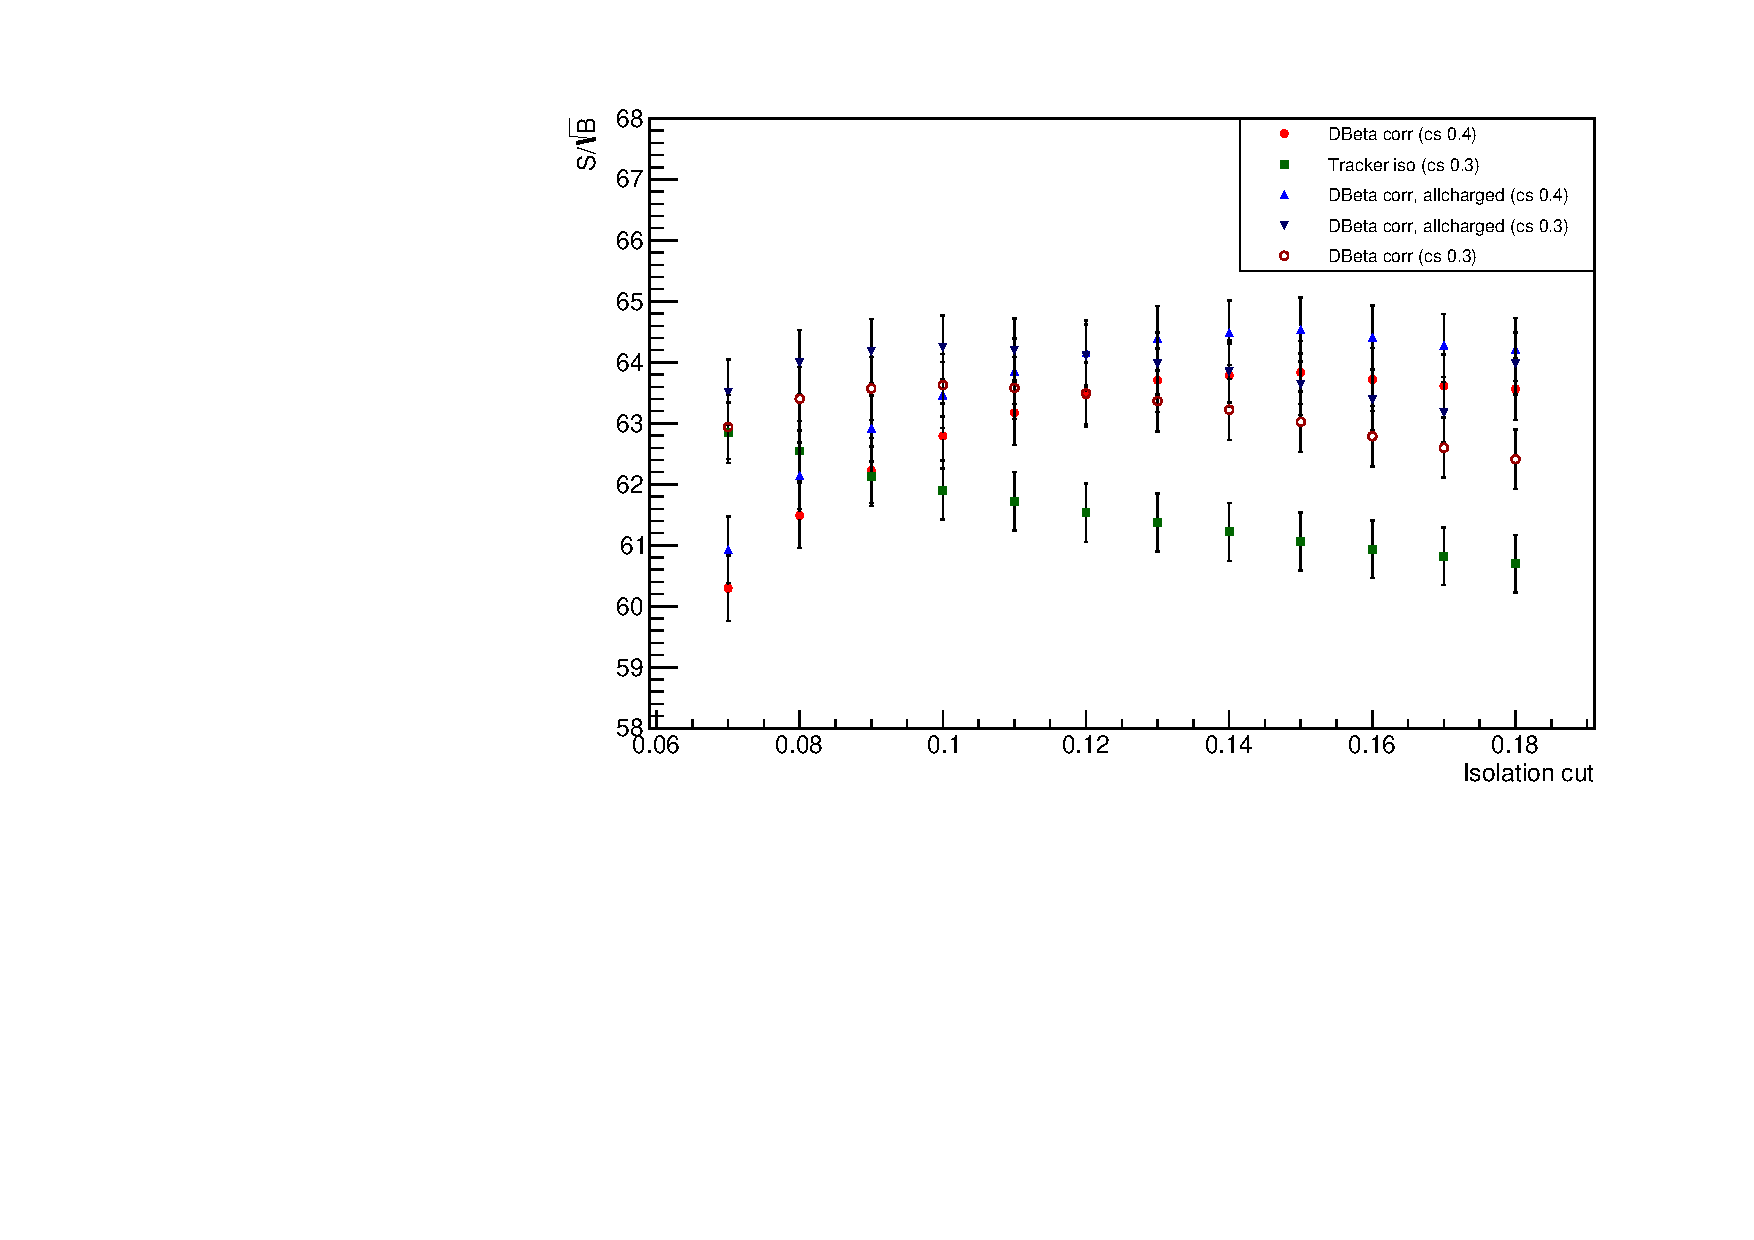
\includegraphics[width=0.7\textwidth]{./MSSM/Figures/s_over_root_b_mt_m.pdf}}~\\
\subfloat[Size of error interval]{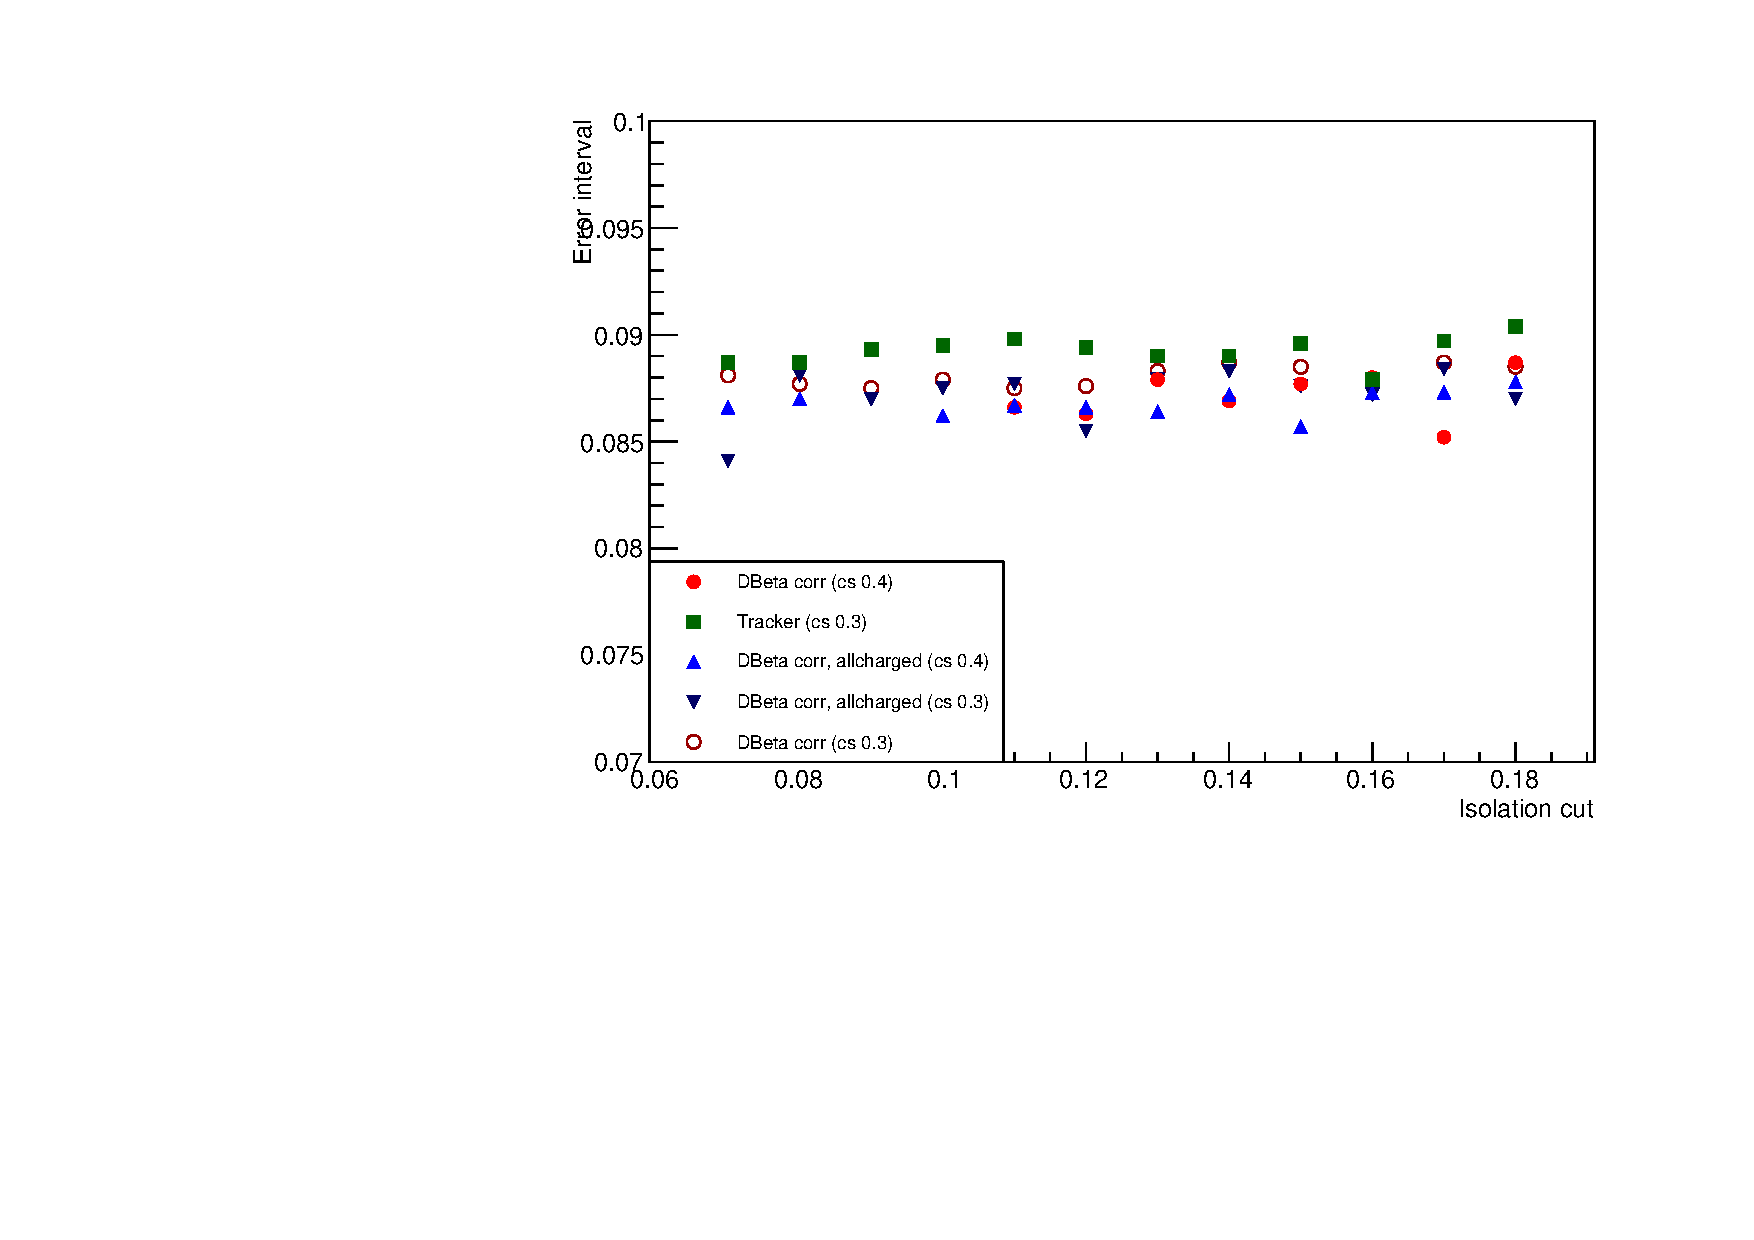
\includegraphics[width=0.7\textwidth]{./MSSM/Figures/mt_muons_iso_errint.pdf}}
\end{center}
\caption{(a) The $S/\sqrt{B}$ for \Ztautau signal and (b) the size of the error interval on 
the best--fit value of a maximum--likeihood fit to the \Ztautau signal strength,
for various cut values of the $\Delta\beta$--corrected
isolation variable with a cone size of $\Delta R = 0.4$ (solid circles), 
the $\Delta\beta$--corrected isolation variable with a cone size of $\Delta R = 0.3$ (open circles),
the $\Delta\beta$--corrected isolation variable including electrons and muons in the isolation
sum, for a cone size of $\Delta R =0.4$ (upward facing triangles) and $\Delta R =0.3$ (downward facing triangles) and
the tracker--based relative isolation (solid squares).}
\label{fig:mssm_selection_mt_muons}
\end{figure}

A topological selection on the \mT~variable, 
introduced in section \ref{sec:hhh_selection_categories}, is made on 
events in the \mutau channel. This selection and the
choice of hadronic tau isolation working point interfere 
with each other and therefore they are optimised in a 2D--optimisation. 
The pre--fit expected upper limits on $\sigma\times$BR for both gg$\phi$ and bb$\phi$
production with decay into $\Pgt\Pgt$ at several mass points 
in the 90 GeV -- 3.2 TeV range are used to do this. 
Because of the use of such a wide range of signal masses, it
is not possible to choose a selection that is optimal
for every mass point. This is illustrated in figure \ref{fig:mssm_selection_mt_taumt}:
figure \ref{fig:mssm_selection_mt_taumt}a shows the upper limit on $\sigma\times$BR for
the gluon--gluon fusion production process, at a mass $m_{\phi} = 160$ GeV, with
figures \ref{fig:mssm_selection_mt_taumt}b,c and d showing this upper limit at $m_{\phi} = 900$ GeV,
$m_{\phi} = 1600$ GeV and $m_{\phi} = 2900$ GeV respectively. From these figures
we can observe that looser selections are preferred for higher masses. This can be
explained by considering the function of each of the selections. Tightening the hadronic
tau isolation working point reduces the selection of fake taus and increases the proportion
of backgrounds which contain real hadronic taus. The \mT~selection reduces
the \Wjets background. As the backgrounds are concentrated at the lower
end of the spectrum of mass--like discriminating variables, such tighter
selections are preferred where signal and backgrounds overlap. However, at higher
mass points the signal--sensitive range of the discriminating variable is 
low in backgrounds and there is more benefit to loosening the selection
to increase the signal efficiency than to keep the tighter selection
to reduce an already low background.

\begin{figure}[h!]
\begin{center}
\subfloat[$m_{\phi} = 160$ GeV]{\includegraphics[width=0.5\textwidth]{./MSSM/Figures/optimisation_ggh_mt_160.0_range12.pdf}}
\subfloat[$m_{\phi} = 900$ GeV]{\includegraphics[width=0.5\textwidth]{./MSSM/Figures/optimisation_ggh_mt_900.0_range12.pdf}}~\\
\subfloat[$m_{\phi} = 1600$ GeV]{\includegraphics[width=0.5\textwidth]{./MSSM/Figures/optimisation_ggh_mt_1600.0_range12.pdf}}
\subfloat[$m_{\phi} = 2900$ GeV]{\includegraphics[width=0.5\textwidth]{./MSSM/Figures/optimisation_ggh_mt_2900.0_range12.pdf}}
\end{center}
\caption{Pre--fit expected limit on $\sigma\times$BR for the gg$\phi$ production process with decay into $\Pgt\Pgt$,
s a function of tau isolation working point (from very loose to very very tight) and
of \mT~ cut from \mT$<20$ GeV to \mt$<40$ GeV, normalised to the best limit in the plane, indicated by the asterisk. This is shown
for $m_{\phi}$ = 160 GeV (a), 900 GeV (b), 1600 GeV (c) and 2900 GeV (d). The most optimal combination of \mT~selection and 
hadronic tau isolation working point varies by mass point, with looser selections preferred for higher masses.}
\label{fig:mssm_selection_mt_taumt}.
\end{figure}

Based on this information, for the analysis on the 2015 dataset the selection was optimised
for mass points around 700-800 GeV. For the analysis on the 12.9 fb$^{-1}$ collected
in the first half of 2016, the selection was further loosened by 10 GeV in \mT~cut
and one step in hadronic tau isolation working point, to obtain the medium isolation working
point selection combined with a selection on \mT$<40$ GeV.

The choice of the hadronic tau \pT selection is driven by the effect on the low mass region:
raising the \pT selection by 10 GeV from the minimum of 20 GeV does not affect the sensivity
of the analysis for high mass points, while recovering some of the loss of loosening 
tau isolation working point and \mT~cut. This is because when using \pT$>30$ GeV 
fewer background events are selected.





\subsection{\texorpdfstring{Event selection in the \etau channel}{Event selection in the e tau channel}}
\label{sec:mssm_eventsel_et}

\subsection{\texorpdfstring{Event selection in the \tautau channel}{Event selection in the tau tau channel}}
\label{sec:mssm_eventsel_tt}

\subsection{\texorpdfstring{Event selection in the \emu channel}{Event selection in the e mu channel}}
\label{sec:mssm_eventsel_em}

\subsection{Leptonvetos}
\label{sec:mssm_eventsel_leptonvetos}

\subsection{Categorisation}
\label{sec:mssm_eventsel_categories}

NEED FIGURE OF NJETS AND NBJETS WITH SIGNAL ON!

\section{\ac{MC} to data correction factors}
\label{sec:mssm_mccorrs}

\section{Discriminating variable}
\label{sec:mssm_discrvar}

\section{Background estimation}
\label{sec:mssm_bkgs}

\subsection{\texorpdfstring{\mutau and \etau channels}{mutau and etau channels}}
\label{sec:mssm_bkgs_mtet}

\subsubsection{\texorpdfstring{\Ztautau}{Z to tau tau}}
\label{sec:mssm_bkgs_mtet_ztt}

\subsubsection{\texorpdfstring{\Wjets}{W+jets}}
\label{sec:mssm_bkgs_mtet_wjets}

\subsubsection{QCD}
\label{sec:mssm_bkgs_mtet_qcd}

\subsubsection{\texorpdfstring{\ttbar}{ttbar}}
\label{sec:mssm_bkgs_mtet_tt}

\subsubsection{Other backgrounds}
\label{sec:mssm_bkgs_mtet_other}

\subsection{\texorpdfstring{\tautau channel}{tautau channel}}
\label{sec:mssm_bkgs_tt}

\subsubsection{\texorpdfstring{\Ztautau}{Z to tau tau}}
\label{sec:mssm_bkgs_tt_ztt}

\subsubsection{QCD}
\label{sec:mssm_bkgs_tt_qcd}

\subsubsection{\texorpdfstring{\Wjets}{W+jets}}
\label{sec:mssm_bkgs_tt_wjets}

\subsubsection{\texorpdfstring{\ttbar}{ttbar}}
\label{sec:mssm_bkgs_tt_tt}

\subsubsection{Other backgrounds}
\label{sec:mssm_bkgs_tt_other}

\subsection{\texorpdfstring{\emu channel}{emu channel}}
\label{sec:mssm_bkgs_em}

\subsubsection{\texorpdfstring{\Ztautau}{Z to tau tau}}
\label{sec:mssm_bkgs_em_ztt}

\subsubsection{QCD}
\label{sec:mssm_bkgs_em_qcd}

\subsubsection{\texorpdfstring{\Wjets}{W+jets}}
\label{sec:mssm_bkgs_em_wjets}

\subsubsection{\texorpdfstring{\ttbar}{ttbar}}
\label{sec:mssm_bkgs_em_tt}

\subsubsection{Other backgrounds}
\label{sec:mssm_bkgs_em_other}


\section{Systematic uncertainties}
\label{sec:mssm_uncs}

\subsection{Normalisation uncertainties}
\label{sec:mssm_uncs_norm}

\subsection{Shape uncertainties}
\label{sec:mssm_uncs_shape}

\section{Signal extraction}
\label{sec:mssm_signalextraction}

\subsection{Inclusion of control regions in the fit}
\label{sec:mssm_sigext_ctrl}

\section{Results}
\label{sec:mssm_results}

\subsection{Model--independent results}
\label{sec:mssm_results_modelindep}

\subsection{Interpretation in MSSM benchmark scenarios}
\label{sec:mssm_results_modeldep}

\section{Combination of 2015 and 2016 datasets}
\label{sec:mssm_combination}

\subsection{Procedure}
\label{sec:mssm_combination_procedure}

\subsection{Results}
\label{sec:mssm_combination_results}


